\documentclass{exam}

\usepackage{units} 
\usepackage{graphicx}
\usepackage[fleqn]{amsmath}
\usepackage{cancel}
\usepackage{float}
\usepackage{mdwlist}
\usepackage{booktabs}
\usepackage{cancel}
\usepackage{polynom}
\usepackage{caption}
\usepackage{fullpage}
\usepackage{xfrac}
\usepackage{enumerate}

\newcommand{\dg}{\ensuremath{^\circ}} 
\everymath{\displaystyle}

\printanswers

\title{Math 142 Notes \\ Section 7.1}

\date{\today}

\begin{document}

  \maketitle
  \tableofcontents

  \section{Identities}
  \subsection{Pythagorean Identities}
  \begin{align*}
    \sin^2 x + \cos^2 x & = 1 \\
    \tan^2 x + 1        & = \sec^2 x \\
    \cot^2 x + 1        & = \csc^2 x \\
  \end{align*}

  \subsection{Even/Odd Identities}
  \begin{align*}
    \sin(-x) & = - \sin x \\
    \cos(-x) & = \cos x \\
    \tan(-x) & = - \tan x \\
  \end{align*}

  Show with:
  \begin{itemize*}
    \item unit circle
    \item y-axis (cosine) or origin (sine and tangent) symmetry in graph
  \end{itemize*}

  \subsection{Cofunction Identities}
  \begin{align*}
    \sin \left( \frac{\pi}{2} - u \right) &= \cos u \\
    \cos \left( \frac{\pi}{2} - u \right) &= \sin u \\
    \tan \left( \frac{\pi}{2} - u \right) &= \cot u \\
    \\
    \sec \left( \frac{\pi}{2} - u \right) &= \csc u \\
    \csc \left( \frac{\pi}{2} - u \right) &= \sec u \\
    \cot \left( \frac{\pi}{2} - u \right) &= \tan u \\
  \end{align*}

  Show with right triangle.

  Show with graph reflection:

  \begin{figure}[H]
    \centering
    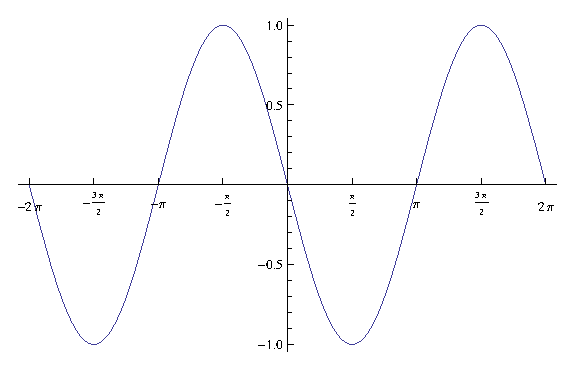
\includegraphics[scale=0.7]{sine_negative_x}
    \caption{$g(x) = \sin(-x)$}
  \end{figure}

  \begin{figure}[H]
    \centering
    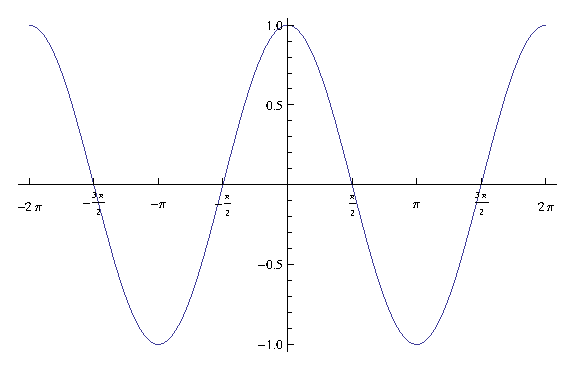
\includegraphics[scale=0.7]{cosine_x}
    \caption{$g(x - \sfrac{\pi}{2}) = \sin(- ( x - \sfrac{\pi}{2}))$}
  \end{figure}

  \begin{figure}[H]
    \centering
    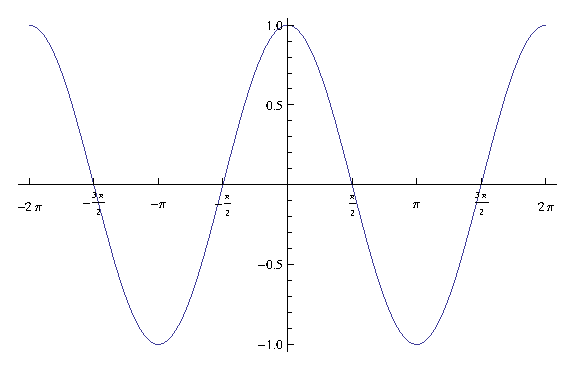
\includegraphics[scale=0.7]{cosine_x}
    \caption{$g(x) = \cos(-x)$}
  \end{figure}

  \begin{figure}[H]
    \centering
    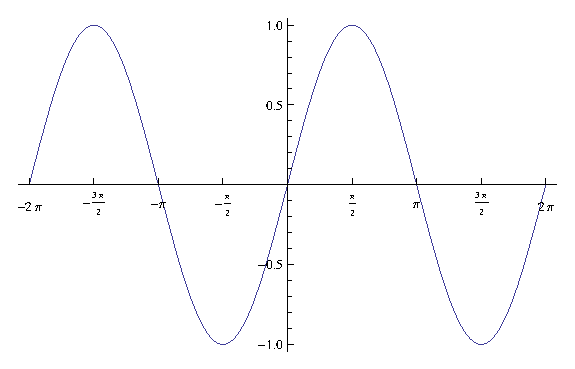
\includegraphics[scale=0.7]{sine_x}
    \caption{$g(x - \sfrac{\pi}{2}) = \cos(- ( x - \sfrac{\pi}{2}))$}
  \end{figure}

  \section{Proving Identities}
  \subsection{Procedure}
  \begin{itemize*}
    \item start with more complicated side
    \item use identities and algebra to simplify
    \item when in doubt, convert everything to sine/cosine
    \item multiplying $(a + b)$ by $(a - b)$ to get $a^2 - b^2$ is sometimes useful
  \end{itemize*}

  \section{Examples}
  \subsection{Simplify}
  \begin{description}

    \item[15]
      \begin{align*}
        \frac{\sec^2 x - 1}{\sec^2 x} & = \tan^2 x \cdot \cos^2 x \\
                                      & = \sin^2 x \\
      \end{align*}

    \item[16] 
      \[
        \frac{\sec x - \cos x}{\tan x} = \sin x
      \]

    \item[17] 
      \begin{align*}
        \frac{1 + \csc x}{\cos x + \cot x} & = \frac{1 + \sfrac{1}{\sin x}}{\cos x + \sfrac{\cos x}{\sin x}} \\
                                           & = \frac{\sin x + 1}{\sin x \cos x + \cos x} \\
                                           & = \sec x \\
      \end{align*}

    \item[18] 
      \begin{align*}
        \frac{\sin x}{\csc x} + \frac{\cos x}{\sec x} &= 1 \\
      \end{align*}

    \item[19] 
      \begin{align*}
        \frac{1 + \sin u}{\cos u} + \frac{\cos u}{1 + \sin u} & = \frac{1 + 2 \sin u + \sin^2 u + \cos^2 u}{\cos u (1 + \sin u)} \\
                                                              & = \frac{2(1 + \sin u)}{\cos u (1 + \sin u)} \\
                                                              & = 2 \sec u \\
      \end{align*}


  \end{description}

  \subsection{Verify the Identity}
  \begin{description}

    \item[25]
      \[
        \frac{\sin \theta}{\tan \theta} = \cos \theta
      \]

    \item[26]
      \[
        \frac{\tan x}{\sec x} = \sin x
      \]

    \item[27]
      \[
        \frac{\cos x \sec x}{\tan x} = \cot x
      \]

    \item[28]
      \[
        \frac{\cot x \sec x}{\csc x} = 1
      \]

    \item[29]
      \[
        \frac{\tan x}{\csc x} = \sec x - \cos x
      \]

    \item[35]
      \[
        \tan x + \cot x = \sec x \csc x
      \]

    \item[36]
      \[
        (\sin x + \cos x)^2 = 1 + 2 \sin x \cos x
      \]

    \item[37]
      \[
        (1 - \cos x)(1 + \cos x) = \frac{1}{\csc^2 x}
      \]

    \item[38]
      \[
        \frac{\cos x}{\sec x} + \frac{\sin x}{\csc x} = 1
      \]

    \item[39]
      \[
        \frac{(\sin x + \cos x)^2}{\sin^2 x - \cos^2 x} = \frac{\sin^2 x - \cos^2 x}{(\sin x - \cos x)^2}
      \]

    \item[45]
      \[
        (\cot x - \csc x)(\cos x + 1) = - \sin x
      \]

    \item[46]
      \[
        \sin^4 x - \cos^4 x = \sin^2 x - \cos^2 x
      \]

    \item[47]
      \[
        \left( 1 - \cos^2 x \right)\left( 1 + \cot^2 x \right) = 1
      \]

    \item[48]
      \[
        \cos^2 x - \sin^2 x = 2 \cos^2 x - 1
      \]

    \item[49]
      \[
        2 \cos^2 x - 1 = 1 - 2 \sin^2 x
      \]

    \item[55]
      \[
        \frac{\sin x - 1}{\sin x + 1} = \frac{- \cos^2 x}{(\sin x + 1)^2}
      \]

  \end{description}
  \section{Trigonometric substitution}
  See exercises 89-94.  


\end{document}
